\Chapter{Szimuláció}


\section{Adatbázisok és modellek}
A programban a drón, és telemetria adatmodell a legfontosabb.
Ezeket az adatokat olvassuk és mentjük,illetve szükségesek az azonosításhoz vagy bármilyen értelmes következtetéshez a problémához kapcsolódóan.

\subsection{Modellek az adatközpont programban}
\subsubsection{Telemetria modell}
A programban a telemetria modell a következőképpen néz ki:

\begin{python}
    package models

    import "time"

    type Telemetry struct {
        Speed              float64          `json:"speed" db:"speed"`
        Location           GPS              `json:"location"`
        Altitude           float64          `json:"altitude"`
        Bearing            float64          `json:"bearing"
        Acceleration       float64          `json:"acceleration"`
        BatteryLevel       int              `json:"battery_level"`
        BatteryTemperature int              `json:"battery_temperature"`
        MotorTemperatures  []int            `json:"motor_temperatures"`
        Errors             []TelemetryError `json:"errors" db:"errors"`
        TimeStamp          time.Time        `json:"time_stamp"`
        DroneID            int              `json:"drone_id"`
    }

    type TelemetryError int

    const (
        MotorFailure TelemetryError = iota
        BeaconSignalStrengthLow
        BeaconSignalInterference
        BeaconTemperatureTooHigh
        GPSInt	eference
        GPSSignalLost
        GPSTemperatureTooHigh
        ProcessorTemperatureTooHigh
        BatteryFailure
        FailedToEjectPackage
        PackageLost
        DestinationDistanceTooFar
    )

    type GPS struct {
        Latitude  float64 `json:"latitude" bson:"latitude"`
        Longitude float64 `json:"longitude" bson:"longitude"`
    }

\end{python}


\subsubsection{Drón modell}
A DDD-ben leírt elvek alapján, a drón modell mindenféleképp egy Entity-nek felel meg.
\begin{python}
    type Drone struct {
        ID           int           `json:"id" db:"drone_id" bson:"id"`
        Telemetry    Telemetry     `json:"telemetry" bson:"telemetry"`
        Parcel       Parcel        `json:"parcel"`
        Destinations []Destination `json:"destinations"`
        Consumption  float64       `json:"consumption"`
        Weight       float64       `json:"weight"`
        State        DroneState    `db:"state" bson:"state"`
    }

    type DroneState string

    const (
    DroneFree     DroneState = "free"
    DroneInFlight DroneState = "in-flight"
    )
\end{python}


\subsubsection{Parcel modell (szállítandó csomag)}
A drónok által szállított csomag így néz ki:
\begin{python}
    type Parcel struct {
        ID            int             `json:"id" db:"id" bson:"id"`
        TrackingID    string          `json:"tracking_id" `
        Name          string          `json:"name" db:"name" bson:"name"`
        Weight        float64         `json:"weight" db:"weight"`
        Location      GPS             `json:"location" bson:"location"`
        FromAddress   ShippingAddress `json:"from_address"`
        ToAddress     ShippingAddress `json:"to_address"`
        DropOffSite   GPS             `bson:"drop_off_site" `
        AssignedDrone int             `json:"assigned_drone" `
    }
\end{python}

\subsection{Relációs adatbázis, PostgreSQL}
A relációs adatbázissal is működik a szimuláció.
\paragraph{Relációs modell \ref{fig:postgres} } \mbox{} \\

\begin{figure}[h]
    \centering
    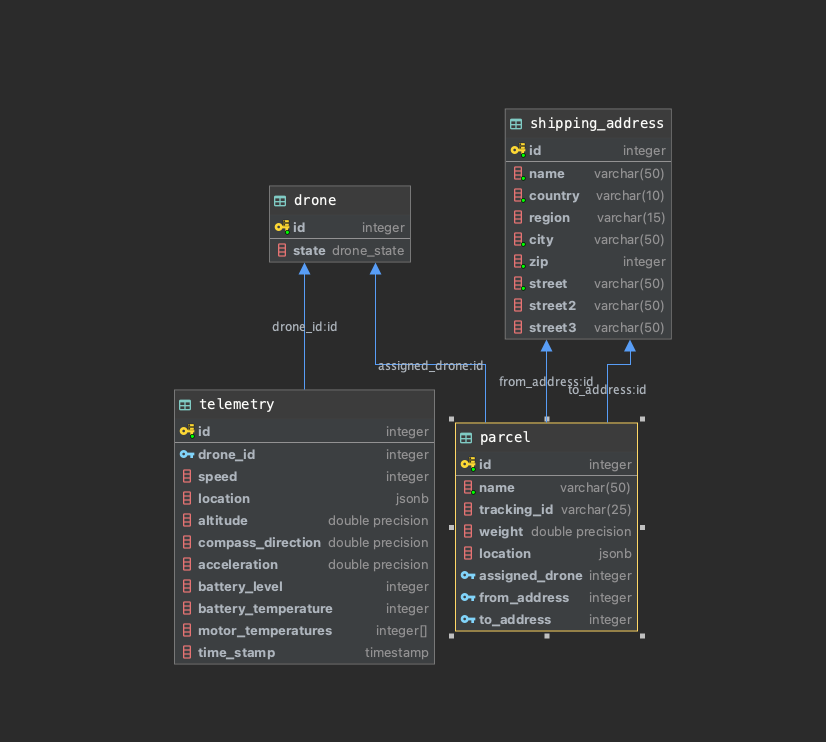
\includegraphics[scale=0.4]{images/postgres.png}
    \caption{PostgreSQL adatbázis modell}
    \label{fig:postgres}
\end{figure}

%TODO: Esetleg Er model


\subsubsection{Lost Update probléma}
A legtöbb relációs adatbázis támogatja a tranzakciókat. A tranzakciók ACID tulajdonságokkal bírnak.
Adatbázisok esetén az ACID az Atomicity (atomiság), Consistency (konzisztencia), Isolation (izoláció), és Durability (tartósság) rövidítése. Ezek nélkül az adatbázis integritása nem garantálható.
A PostgreSQL többféle izolációs szintet biztosít a tranzakciókhoz \cite{postgres-transaction}. A Lost Update problémát garantáltan megoldja a PostgreSQL `Serializable` izolációs szintje.
\begin{table}[h]
    \centering
    \caption{ Standard SQL Transaction Isolation Levels}
    \begin{tabular}{l|c|c|c|}
Isolation Level & Dirty Read  & Nonrepeatable Read & Phantom Read\\
        \hline
Read uncommitted  & Possible & Possible & Possible \\
\hline
Read committed & Not possible & Possible & Possible \\
\hline
Repeatable read & Not possible & Not possible & Possible \\
\hline
Serializable & Not possible & Not possible & Not Possible \\
        \hline
    \end{tabular}
\end{table}

\subsubsection{Telepítése a programhoz}

Az adatbáziskezelőhöz csatlakozva, le kell futtatni a következő SQL scriptet.

\begin{lstlisting}[language=sql]
    CREATE TYPE drone_state AS ENUM ('free', 'in-flight');
    CREATE TABLE drone
    (
    id          SERIAL PRIMARY KEY,
    state       drone_state      DEFAULT 'free',
    weight      DOUBLE PRECISION default 4,
    consumption DOUBLE PRECISION DEFAULT 500
    );

    CREATE TABLE warehouse
    (
    id  SERIAL PRIMARY KEY,
    location_latitude DOUBLE PRECISION DEFAULT 48.080922,
    location_longitude DOUBLE PRECISION DEFAULT 20.766208
    );

    CREATE TABLE shipping_address
    (
    id      SERIAL PRIMARY KEY,
    name    VARCHAR(50) NOT NULL,
    country VARCHAR(10) NOT NULL,
    region  VARCHAR(15) DEFAULT NULL,
    city    VARCHAR(50) NOT NULL,
    zip     INT         NOT NULL,
    street  VARCHAR(50) NOT NULL,
    street2 VARCHAR(50) DEFAULT NULL,
    street3 VARCHAR(50) DEFAULT NULL
    );

    CREATE TABLE parcel
    (
    id                 SERIAL PRIMARY KEY,
    name               VARCHAR(50) NOT NULL,
    tracking_id        VARCHAR(25)               default '',
    weight             DOUBLE PRECISION          default 1,
    drop_off_latitude  DOUBLE PRECISION          DEFAULT 0,
    drop_off_longitude DOUBLE PRECISION          DEFAULT 0,
    assigned_drone     INT REFERENCES drone (id) DEFAULT NULL,
    from_address       INT REFERENCES shipping_address (id),
    to_address         INT REFERENCES shipping_address (id)
    );

    CREATE TABLE telemetry
    (
    id                  SERIAL PRIMARY KEY,
    drone_id            INT REFERENCES drone (id),
    speed               DOUBLE PRECISION DEFAULT 0,
    latitude            DOUBLE PRECISION DEFAULT 0,
    longitude           DOUBLE PRECISION DEFAULT 0,
    altitude            DOUBLE PRECISION default 1,
    bearing             DOUBLE PRECISION DEFAULT 0,
    acceleration        DOUBLE PRECISION DEFAULT 0,
    battery_level       INT              DEFAULT NULL,
    battery_temperature INT              DEFAULT NULL,
    motor_temperatures  INTEGER[],
    errors              INTEGER[],
    time_stamp          timestamp        DEFAULT NULL
    );
    INSERT INTO warehouse (id) VALUES (1);
\end{lstlisting}


\subsection{Dokumentum alapú adatbázis, MongoDB}

\subsubsection{Vizualizáció}

\begin{figure}[hbt!]
    \centering
    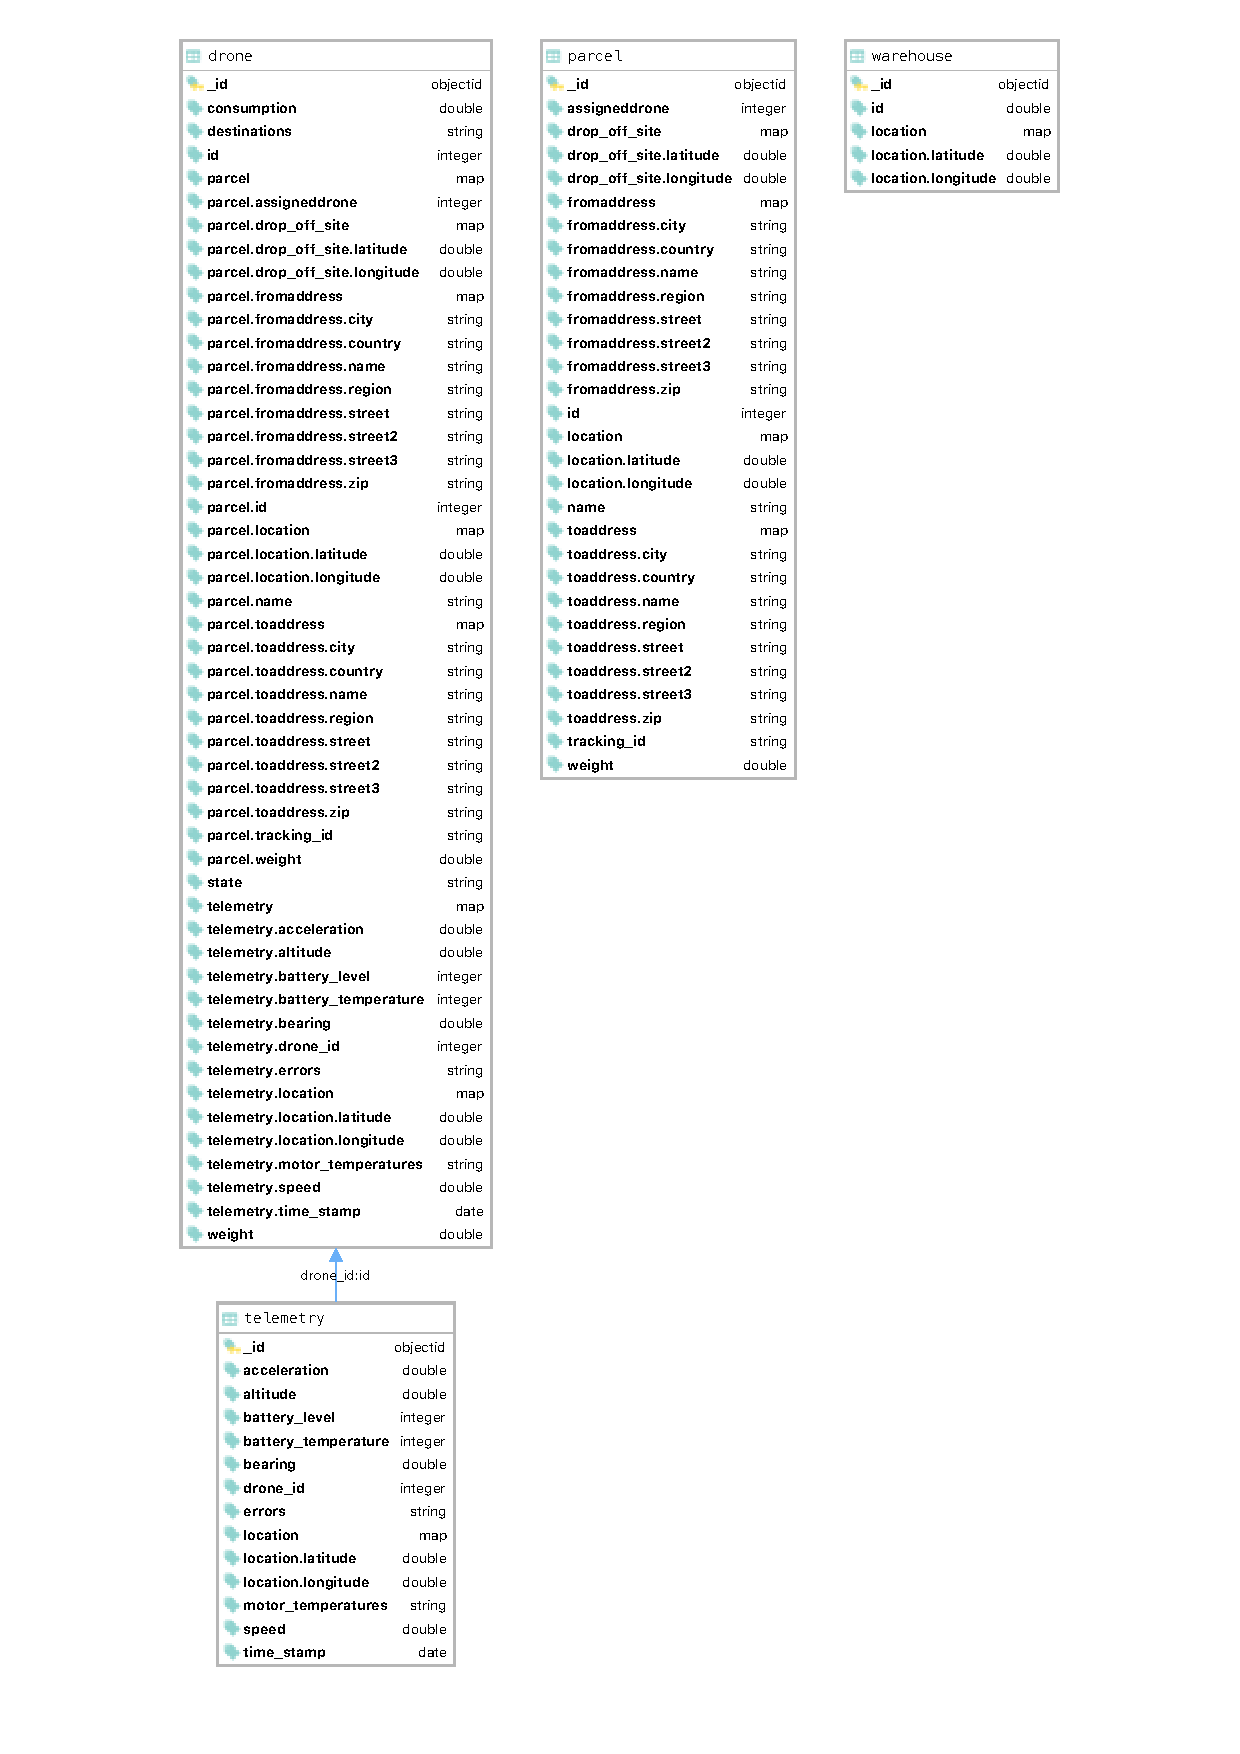
\includegraphics[scale=0.7]{images/mongo.pdf}
    \caption{MongoDB adatbázis vizualizáció}
    \label{fig:mongodb}
\end{figure}

\subsubsection{Telepítése a programhoz}
Az adatbáziskezelő konzolján keresztül le kell futtatni a következő két parancsot, egy megfelelő jogosultságú felhasználóval.
Ez egyik parancs létrehozza a drone\_delivery adatbázist, a másik parancs létrehoz nekünk egy felhasználót az előbb létrehozott adatbázishoz.
A későbbiekben ezzel a felhasználóval csatlakozunk az adatbázishoz.

\begin{python}
    use drone_delivery
\end{python}

\begin{python}

    db.createUser(
        {
        user: "drone-user",
        pwd: "drone-pwd",
        roles: [
            {
            role: "readWrite",
            db: "drone_delivery"
        }
        ]
    }
    )
\end{python}



\section{A rendszer felépítése a követelmények alapján}
%TODO: ide irni Hexagonal arch. es DDD implementaciojarol. Beszurni kodot ahol latszik a repository, interface
\subsubsection{Szerkezeti felépítés}
Az alkalmazás jegyzék struktúráját a következő ábra \ref{fig:szerkezet} mutatja.
A drone-delivery jegyzék a program gyökér jegyzéke, itt található a docker-compose.yml fájl, ami az indításhoz szükséges.
A backend/server tartalmazza az adatközpont programot és a backend/drone-swarm a drón-raj programot.
Mindkét jegyzéknek hasonló a felépítése.
A cmd jegyzékbe van az indító main függvény.
A pkg jegyzék tartalmazza a kódbázis nagy részét, a domain és infrastuktúrához kapcsolódó részek itt helyezkednek el.
A pkg/domain/ben a domain kódbázis található, az infrastruktúrát és a hozzá tartozó adaptereket megvalósító kód a storage, network jegyzékekben van.
A drone-delivery/web-clientben található a web kliens, egy egyszerű html oldal ahonnan beállítjuk a szimulációt.

\begin{figure}[h]
    \centering
    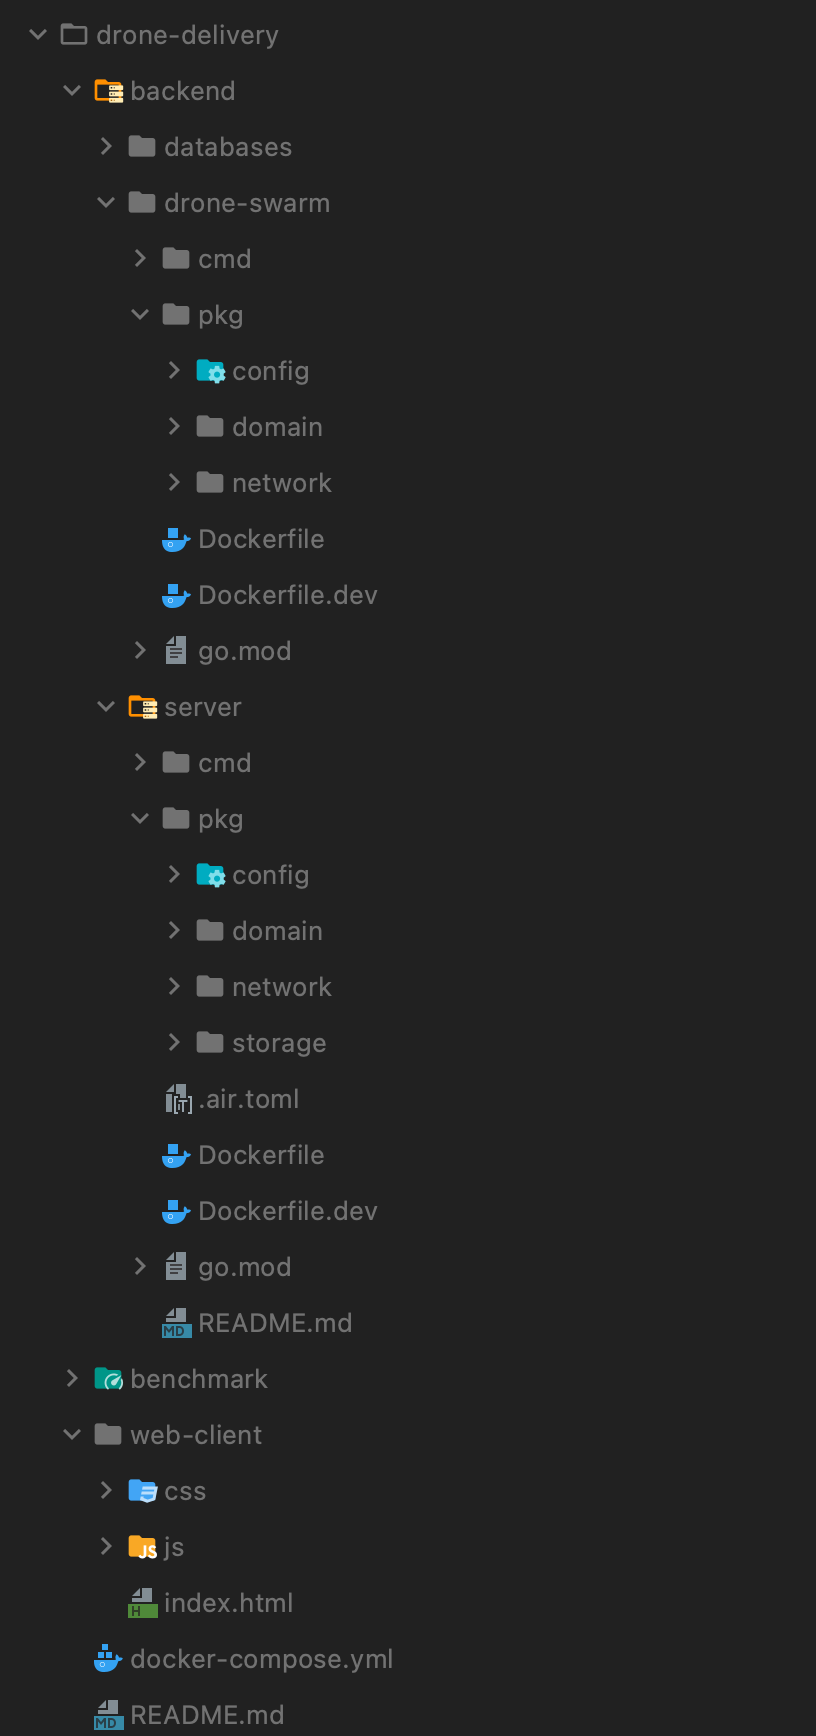
\includegraphics[scale=0.5]{images/szerkezet}
    \caption{Jegyzék szerkezet}
    \label{fig:szerkezet}
\end{figure}

\subsubsection{Portok és Adapterek, Domain Driven Design}
A hexagonal tervezési architektúra mindkét programban úgy került implementálásra, hogy a program magja, a domain üzleti logika a pkg/domain jegyzékben helyezkedik el.
Ez a domain jegyzék modellezi le az üzleti logika működését.
Itt találhatóak az interfészek, amik a hexagonal architektúra portjaiként szolgálnak, ezt kell implementálniuk az adaptereknek, így van összekötve a domain a különböző adapterekkel.
A DDD elemeit is megfigyelhetjük az elnevezésekből, valamint vannak Entity-k és Value Objectek.
\begin{python}
    # Entity
    type Drone struct {
        ID           int           `json:"id" db:"drone_id" bson:"id"`
        Telemetry    Telemetry     `json:"telemetry" bson:"telemetry"`
        Parcel       Parcel        `json:"parcel"`
        Destinations []Destination `json:"destinations"`
        Consumption  float64       `json:"consumption" db:"consumption" bson:"consumption"`
        Weight       float64       `json:"weight" db:"weight" bson:"weight"`
        State        DroneState    `db:"state" bson:"state"`
    }

    # Value Object
    type Destination struct {
        Coordinates          GPS
        ParcelDestination    bool
        WarehouseDestination bool
    }

    # Value Object
    type GPS struct {
        Latitude  float64 `json:"latitude" bson:"latitude"`
        Longitude float64 `json:"longitude" bson:"longitude"`
    }
\end{python}

\paragraph{Portok}\mbox{} \\
Minden szervízhez tartozik interface (port) amin az adapterek vagy más szervízek meghívhatják a szervíz metódusait.
Például az adatközpont drón szervízében olyan metódusok találhatóak amiket a REST API hív meg.
Itt a REST API az adapter, pontosabban vezérlő adapter.

\begin{python}
    type Service interface {
        DeliverParcels() error
        ProvisionDrone(wh models.Warehouse, d models.Drone) error
        GetFreeDrones() ([]models.Drone, error)
        GetDronesDelivering() ([]models.Drone, error)
        ChangeService(r Repository)
        ReinitializeDatabase(repos ...Repository) error
    }
\end{python}
Vezérelt adaptere az adatbázist és kimenő kommunikációt megvalósító adapterek.
Az adatközpon programban az adatbázisoknak a Repository interfészt kell implementálni, de a gRPC és JSON kommunikációhoz is tartozik interfész.
\begin{python}
    type Repository interface {
        GetFreeDrones() ([]models.Drone, error)
        GetParcelsInWarehouse() ([]models.Parcel, error)
        GetWarehouse() (models.Warehouse, error)
        GetDronesDelivering() ([]models.Drone, error)
        SetDroneState(droneID int, state string) error
        ReInitializeDeliveryData(drones []models.Drone, parcels []models.Parcel) error
    }

    type OutboundAdapter interface {
        FetchProvisionDroneEndpoint(wh models.Warehouse, d models.Drone) (success bool, err error)
    }
\end{python}

Ugyanígy a drón-raj programban.
\begin{python}
    type OutboundAdapter interface {
        SendTelemetryDataToServer(t models.Telemetry) error
    }
\end{python}
\paragraph{Adapterek} \mbox{} \\
Az adaptereket a portokon keresztül érjük el.
Alább a drón-raj program OutboundAdapter interfészét megvalósító adapter implementációját látjuk, gRPC-vel.
Csak azokat a részeket tartalmazza a példa ami szükséges a megértéshez.
Mivel a "SendTelemetryDataToServer(t models.Telemetry) error " metódus megtálható az adapterben, az interfész teljesül és az adapter használható a porton keresztül.
\begin{python}
    package grpc
    ...
    type Adapter struct {
        cc  *grpc.ClientConn
        tsc protobuf.TelemetryServiceClient
        streams map[int]StreamClient
    }

    func NewOutBoundAdapter() *Adapter {
        ...
    }

    func (a *Adapter) SendTelemetryDataToServer(t models.Telemetry) error {
        var err error
        var streamer protobuf.TelemetryService_TelemetryStreamClient
        ...
        telemetryDataRequest := protobuf.TelemetryDataRequest{
            Telemetry: &protobuf.Telemetry{
                Speed: t.Speed,
                Location: &protobuf.GPS{
                    Latitude:  t.Location.Latitude,
                    Longitude: t.Location.Longitude,
                },
                Altitude:           t.Altitude,
                Bearing:            t.Bearing,
                Acceleration:       t.Acceleration,
                BatteryLevel:       int32(t.BatteryLevel),
                BatteryTemperature: int32(t.BatteryTemperature),
                MotorTemperatures:  temperatures,
                Errors:             telemetryErrors,
                TimeStamp:          timestamppb.New(t.TimeStamp),
                DroneId:            int32(t.DroneID),
            },
        }
        err = streamer.Send(&telemetryDataRequest)
    }

\end{python}

Az adatközpont program adatbázist megvalósító adapterek a pkg/storage jegyzékben helyezkednek el. Itt találhatjuk a MongoDB és PostgreSQL adatbázist használó adaptereket.


\subsubsection{Dependency Injection}
%TODO: szekvencia diagramok is a mukodesrol, a kodban. Main fgv. -> newservice ... -> rest es grpc endpoint




\section{Az rendszer működése}

%TODO: brew services start mongodb-community@4.4, Postgres inditasa
%TODO: Docker, elindul, milyen servicek vannak, mit csinalnak stb.

\section{Szállítási probléma a programban}
\subsubsection{Az adatközpont távolság számítása}
Az adatközpont program az Ortodroma számítást használja, hogy kiszámolj a távolságot a legoptimálisabb útvonal keresése közben.
\begin{python}
    func (s *service) CalculateDistance(lat1, lng1, lat2,
    lng2 float64, unit ...string) float64 {
        const PI = float64(math.Pi) //3.141592653589793

        radlat1 := PI * lat1 / 180
        radlat2 := PI * lat2 / 180

        theta := lng1 - lng2
        radtheta := PI * theta / 180

        dist := math.Sin(radlat1)*math.Sin(radlat2) +
        math.Cos(radlat1)*math.Cos(radlat2)*math.Cos(radtheta)

        if dist > 1 {
            dist = 1
        }

        dist = math.Acos(dist)
        dist = dist * 180 / PI
        dist = dist * 60 * 1.1515

        if len(unit) > 0 {
            if unit[0] == "K" {
                dist = dist * 1.609344
            } else if unit[0] == "N" {
                dist = dist * 0.8684
            } else if unit[0] == "METER" {
                dist = dist * 1.609344 * 1000
            }
        }

        return dist
    }
\end{python}
\subsubsection{A drón-raj program számításai}
A pontos szimulációs értékekhez egy könyvtárat használunk, ami megfelel a WGS84 GPS rendszernek.
Ezzel a könyvtárral pontos adatokat tudunk generálni a drón helyzetéről, irányáról.

\begin{python}

    geo := ellipsoid.Init("WGS84", ellipsoid.Degrees, ellipsoid.Meter,
    ellipsoid.LongitudeIsSymmetric, ellipsoid.BearingIsSymmetric)
    routingService := routing.NewService(geo)

\end{python}

Ezután a útvonalakért felelős szervízben két metódussal számoljuk ki a szükséges értékeket.
A \textit{CalculateDroneDistanceAndDirectionFromDestination} metódussal adott induló koordináták alapján megkapjuk a legrövidebb utat a célkoordinátákhoz, és az irányt is.
A \textit{CalculateDroneNextCoordinates} metódus megmondja adott induló koordináták és távolság valamint irány alapján hogy hova érkezünk, azaz a célkoordinátákat.

\begin{python}
    func (s *service) CalculateDroneDistanceAndDirectionFromDestination(
    currentLat, currentLon, destinationLat, destinationLon float64)
    (distance, bearing float64) {
        distance, bearing = s.geometry.To(currentLat,
        currentLon, destinationLat, destinationLon)
        return distance, bearing
    }

    func (s *service) CalculateDroneNextCoordinates(lat, lon,
    dist, bearing float64) (nextLat,nextLon float64) {
        nextLat, nextLon = s.geometry.At(lat, lon, dist, bearing)
        return nextLat, nextLon
    }
\end{python}

\Section{Benchmarkok}

%hogy hogyan is lesz mikroszerviz. Go kit ben van service discovery,  beepitett Observability (Prometheus), többszintes logger, és A hexagonal architektúrát támogatja
%Pl más hasonló mikroszervizeket kezelő framework (pl. Micro) nem elég rugalmas, sok mindent nem enged meg, egy féleképpen lehet használni.
